
\section{Evaluation of Project}
Evaluation of the project consisted of multiple stages ranging from verification of the functional requirements through simple black box testing to evaluation of refined mesh quality using methods provided by Dittmer \cite{DittmerMeshQualityMet}. 

\subsection{Validation against Functional Requirements}
In order to validate the system against many of the functional requirements the system only needs to be run on several basic models with different input configurations. 

% this
output clearly demonstrates the systems ability to evaluate the quality of meshes using a range of metrics and refinement occurring as a result of both the stresses induced by the user and on their categorisation of edges. 

\subsection{Unit Testing}
Holistic evaluation provided evidence of the overall systems effectiveness however without verification of individual components used to 




\subsection{Validation against Non Functional}
Validation of non functional requirements was made simple due to the limited number of them, this was partly a consequence of the system not being designed for a specific user base resulting in expectations regarding the systems design to improve usability and guide interaction. It was also not possible to define the general accuracy and performance of the system during the requirement elicitation phase since this could only be determined once the required research and trial on the finished system gave indication to both of these. \\


\noindent
In the case of quality for the systems design and documentation evidence is present to indicate that this adheres to the requirements specified with the project submission containing detailed documentation in the form of a Deoxygen guide and sophisticated use of object oriented and functional software design as seen within the codebase. General applicability of functionality has also been demonstrated through evaluation using a variety of both models and conditions when performing simulations.

\subsection{Evaluation Of The system For Various Models}

%To demonstrate the systems applicability to a variety of real engineering problems demanded the creation of several models resembling basic equivalents of real structures that are often analysed by FE methods.

several models have been created resembling basic equivalents of that used for real engineering applications.

 do this reliably and validate the heuristic component against the results obtained in academic papers two of the three models were based on those previously used by Dolsak (Paper mill and Cylinder structures). In addition to these two a suspension bridge model was developed to demonstrate the systems capacity to work beyond Dolsaks basic validation examples. \\ 

\noindent
These initial models were constructed manually using LISA's graphical user interface using measurements by Dolsak and in the case of the suspension bridge from documents available on the web \cite{DolsakPaper91} \cite{SuspensionBridgeMeasurements}.

\subsubsection{Suspension Bridge structure}


\noindent
The basic bridge structure consists of 196 elements and 212 nodes, which is very coarse for a FE mesh structure. \\


\noindent
The primary model for which work on the latter half of the project was based upon was the following suspension bridge model:


\begin{figure}
  \centerline{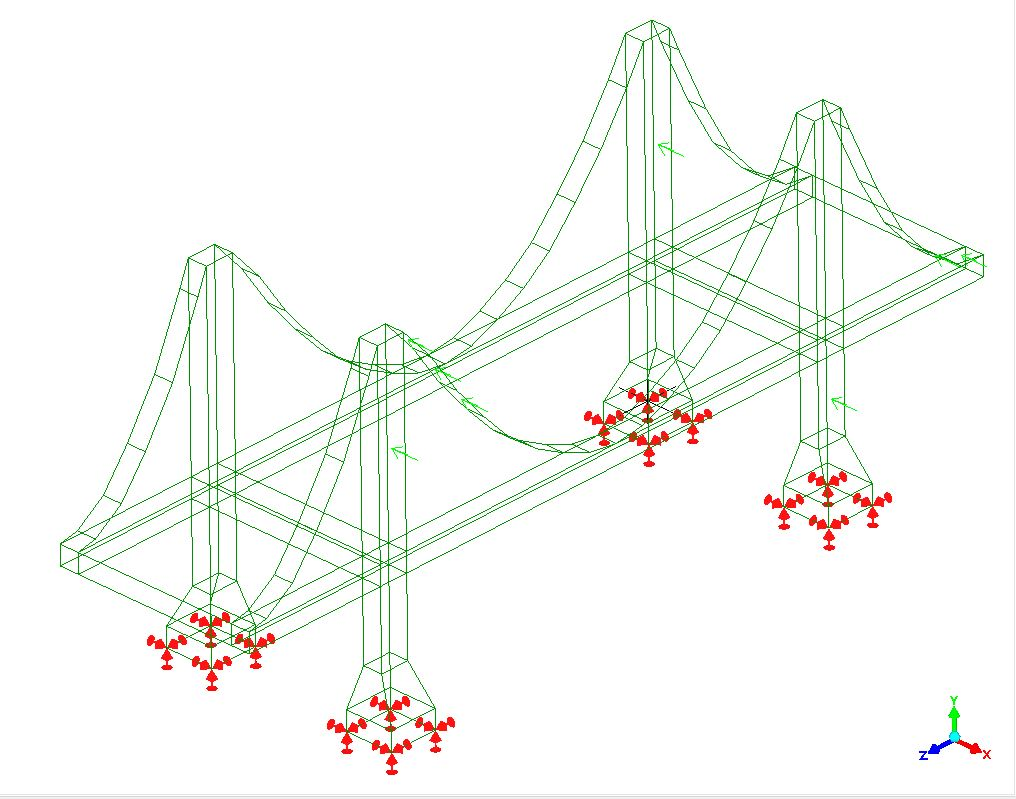
\includegraphics[width=150mm, scale=1]{../Graphics/BasicBridge.jpeg}}
  \caption{Diagram representing the general structure of the system with interactions between non internal entities such as files and LIA shown using dashed lines}
  \label{fig:h-refinementImp}
\end{figure}


\newpage


\noindent
One of the bridge models strengths was it provided high versatility when testing the software solution for m since simulation could be run with forces placed on a range of different faces with corresponding edge rules and a range of varying results obtained. For example a force on the desk of the bridge could be used to simulate the weight of a vehicle moving over it while forces placed sideways on the towers and cables could be used to model stress induced from strong crosswinds.

\subsubsection{Evaluation of bridge for sideways loading}
Simulating effects of forces across the bridge provided an opportunity  to test the system when simulating a scenario that could feasibly effect the structure in the real world such as crosswinds.

%A force was calculated for each section of the bridge when subjected to a crosswind of 70mph, 
% specify formula for calculating cross loadinghttp://www.wikihow.com/Calculate-Wind-Load

%typical significance of crosswinds on suspension bridges
%some general forces and on which part of the bridge are they exerted,
%Image showing the forces placed on the actual bridge and possibly on a diagram from some engineering company.
%Where is stress expected to be induced.
\cite{CrosswindsOnSuspensionBridges}

In order to mesh successfully in order to focus refinement on these areas the following rules can be suggested for the bridge structure when crosswinds are applied from a negative x direction.



\subsubsection{Evaluation of bridge for base loading}
Loading the base of a bridge is yet another typical analysis conducted within civil engineering. The loading can be used to represent anything which moves over the bridge that needs to be supported by it such as vehicles or pedestrians. 


\subsubsection{Validating system against previously obtained research results}
Due to a lack of specific implementation details provided by Dolsak and Muggleton in their papers for generating meshes it was important to demonstrate that the underlying implementation for generating meshes based upon the rules was essentially equivalent. \\ 


Dolsak did however provide information about the various models 

this the models used by Dolsak in order to train his initial ILP system responsible for generating the rules were re crated. This allowed for verification of the heuristic component of the project through comparison of both implentations outputs. \cite{DolsakPaper91}.


\subsubsection{Paper Mill}
Disks are used in multiple places within the paper manufacturing process in order to press the paper as it undergoes pressing and drying. Unlike the bridge example where stresses are for the most part induced by external loading disks within paper mills are primarily stressed as a result of centripetal loading \cite{} Consequently stresses are much more even assuming symmetry in the geometry \cite{RotatingDiskFE}.


Assuming a disk is rotating at a particular speed it is possible to calculate the centrifugal force exerted outwards on it. This has been done in the appendix section for various points on the mill to calculate feasible input for the system \cite{RotatingDiskFE}.



\begin{figure}[!h]
\centering
\begin{subfigure}{.5\textwidth}
  \centering
  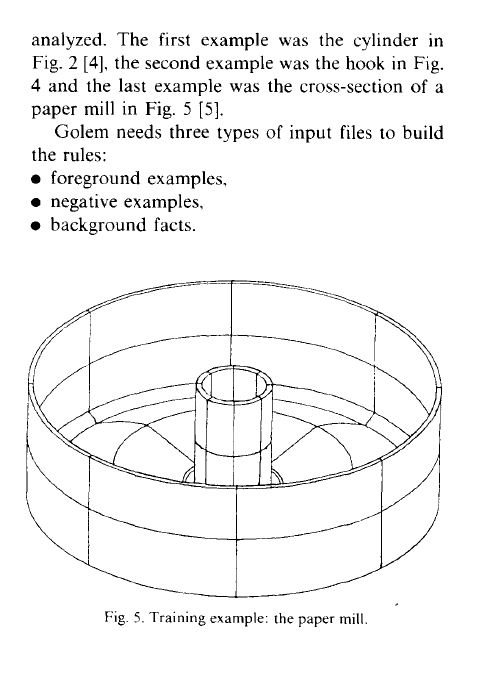
\includegraphics[width=0.9\linewidth]{../Graphics/PaperMillDolsak.jpeg}
  \caption{Paper Mill presented by Dolsak in his paper as input for training Golem}
  \label{fig:sub1}
\end{subfigure}%
\begin{subfigure}{.5\textwidth}
  \centering
  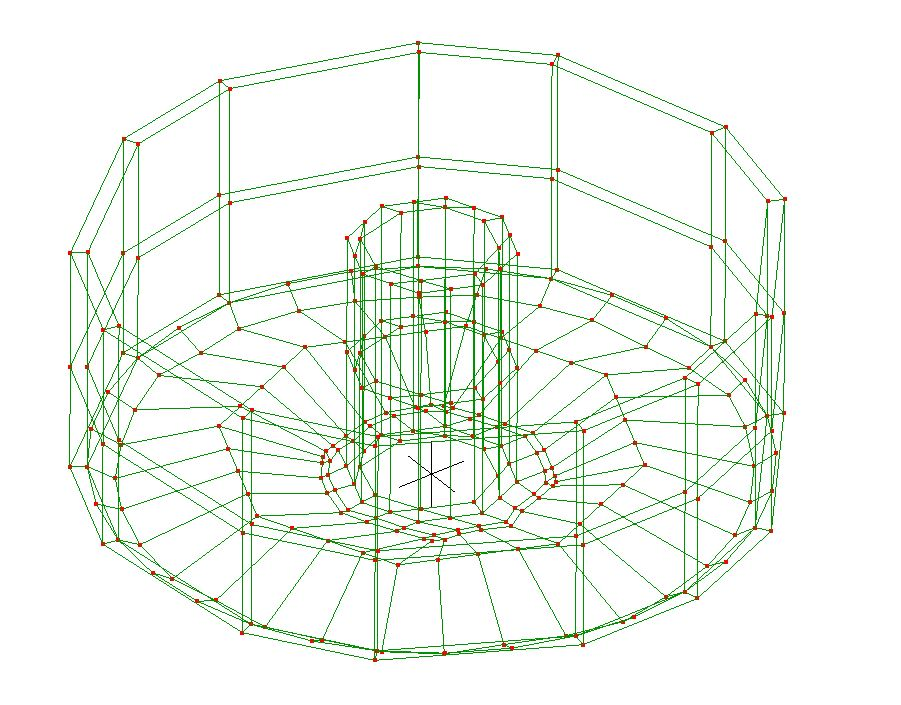
\includegraphics[width=0.9\linewidth]{../Graphics/PaperMillWithinLisa.jpeg}
  \caption{Representation of paper mill within LISA before applying meshing rules to validate}
  \label{fig:sub2}
\end{subfigure}
\label{fig:test}
\end{figure}




\subsubsection{Cylinder}
Obtaining results based on the edge relationships described within the research literature was the first step required when performing evaluation of the cylinder. The rules provided in Dolasks paper used to generate the initial JSON file were the following:




\begin{figure}
\centering
\begin{subfigure}{.5\textwidth}
  \centering
  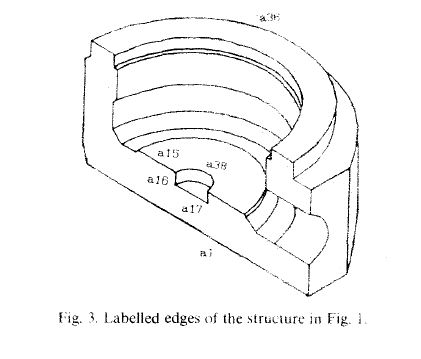
\includegraphics[width=0.9\linewidth]{../Graphics/DolsakCylinderWithEdges.jpeg}
  \caption{Cylinder model used by Dolsak with edges labeled, each labelling corresponds to a rule generated by the Golem algorithm \cite{DolsakPaper91}}
  \label{fig:sub1}
\end{subfigure}%
\begin{subfigure}{.5\textwidth}
  \centering
  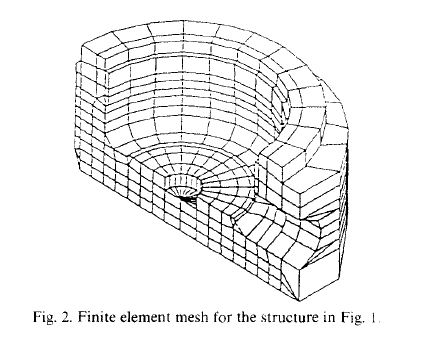
\includegraphics[width=0.9\linewidth]{../Graphics/DolsakCylinderMeshed.jpeg}
  \caption{Diagram representing the general structure of the system with interactions between non internal entities such as files and LIA shown using dashed lines}
  \label{fig:sub2}
\end{subfigure}
\label{fig:test}
\end{figure}

The resulting mesh generated by the system after increasing numbers of iterations based primarily

\begin{figure}
\centering
\begin{subfigure}{.5\textwidth}
  \centering
  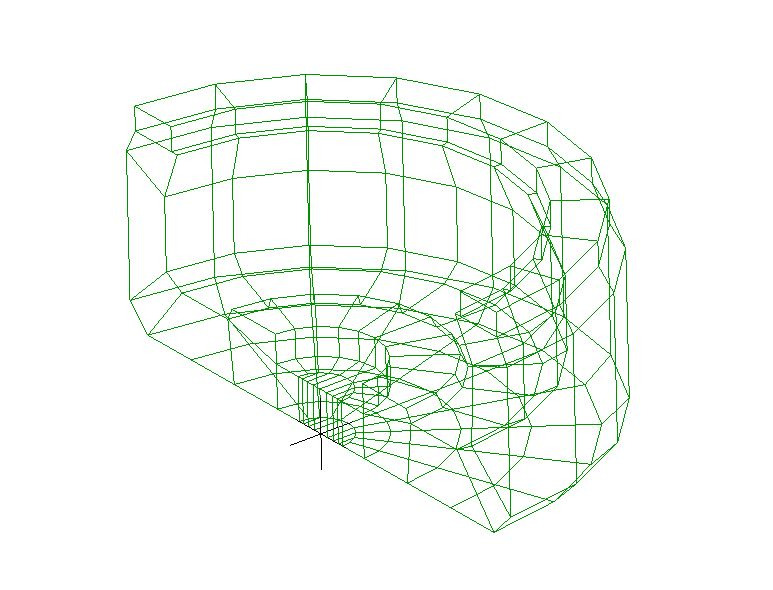
\includegraphics[width=0.9\linewidth]{../Graphics/DolsakCylinderWithinLisa.jpeg}
  \caption{Cylinder cross section initial construction within Lisa \cite{DolsakPaper91}}
  \label{fig:sub1}
\end{subfigure}%
\label{fig:test}
\end{figure}




\newpage
\subsection{Evaluation of Subsystems based on model evaluation}
Having run the system on the range of models described above it was possible to begin assessing it's ability to mesh and the use of Dittmers metrics for assessing 
the quality of each mesh.

\subsubsection{Analysis of Dittmer mesh quality metrics}
When evaluating Dittmers metrics for distinguishing between meshes of different qualities there were several key observations about the metrics in particular which resulted in re assessment of how to evaluate the mesh qualities in general.
Central to these observations was that although metrics provided by Dittmer give a clear indication of the general accuracy of stress across a mesh or a particular element in the majority of cases they give no further insight into the strengths of the particular element arrangement within a given mesh. Consequently it was possible to demonstrate that the meshes produced as a result of the methods retailed general quality that is desired within general meshes but not that the mesh was especially good given the particular model it was based on. \\



%Subsequent research suggested


\subsubsection{Evaluation of stress refinement effectiveness}

\subsubsection{Evaluation of heuristic refinement effectiveness}



\subsection{Increase in performance through parallel execution}
The following 

The average speed up (Time of serial execution/ Time of parallel execution) was 


The Efficiency of the parallel execution (speedup / number of processors) with an Intel i5 processor with 4 cores the average efficiency  was calculated as

\subsection{Quality}
The quality of the design and implementation of the system reflects my experiance not only as a computer science undergraduate but as a developer with one year industrial experience, although not directly effecting the execution of the program properties such as appropriate variable naming, loose coupling of classes, use of abstractions and descriptive error messages make the software easier to read and debug for any potential future developers. 

Using Visual Studio also facilitated calculation of various software quality metrics such as  for the code base automatically. This made it much easier to select parts of the codebase for refactoring when time was allocated for this and 

\subsection{Documentation}
The process of continuously writing descriptive documentation was important to the success of the project and was treated as an integral part to meeting to the goals of the project development methodology which aimed to reduce the systems complexity and improve readability. Through the writing Doc comments corresponding to every function within the codebase it was possible to generate documentation files automatically through use of the tool Doxygen. This allows anyone with the solution to view descriptions of each of its functions either in the codebase or alternatively through the manual produced automatically by Doxygen.

\subsection{Maintainability}
As a result of loosely coupled design with each file containing only one class and each class and function written with the goal of providing only one item of functionality. the 

and well written documentation the system is for the most part maintainable. 


\subsubsection{Evaluation Issues}
A significant issue faced in attempting to demonstrate the effectiveness of the system was to provide an indication of how well the system worked without taking into account the ability of the user who may be providing the edge rules for a particular model. Not taking this into account would result in an inaccurate representation of its ability.

\subsection{Evaluation of overall project}

% Overall the project met all its initial requirements laid out in both the objectives and its requirements.
% 


\subsection{Evaluation summary}
